%
% This is the LaTeX template file for lecture notes for EE 382C/EE 361C.
%
% To familiarize yourself with this template, the body contains
% some examples of its use.  Look them over.  Then you can
% run LaTeX on this file.  After you have LaTeXed this file then
% you can look over the result either by printing it out with
% dvips or using xdvi.
%
% This template is based on the template for Prof. Sinclair's CS 270.

\documentclass[twoside]{article}
\usepackage{graphicx}
\setlength{\oddsidemargin}{0.25 in}
\setlength{\evensidemargin}{-0.25 in}
\setlength{\topmargin}{-0.6 in}
\setlength{\textwidth}{6.5 in}
\setlength{\textheight}{8.5 in}
\setlength{\headsep}{0.75 in}
\setlength{\parindent}{0 in}
\setlength{\parskip}{0.1 in}

%
% The following commands set up the lecnum (lecture number)
% counter and make various numbering schemes work relative
% to the lecture number.
%
\newcounter{lecnum}
\renewcommand{\thepage}{\thelecnum-\arabic{page}}
\renewcommand{\thesection}{\thelecnum.\arabic{section}}
\renewcommand{\theequation}{\thelecnum.\arabic{equation}}
\renewcommand{\thefigure}{\thelecnum.\arabic{figure}}
\renewcommand{\thetable}{\thelecnum.\arabic{table}}

%
% The following macro is used to generate the header.
%
\newcommand{\lecture}[4]{
   \pagestyle{myheadings}
   \thispagestyle{plain}
   \newpage
   \setcounter{lecnum}{#1}
   \setcounter{page}{1}
   \noindent
   \begin{center}
   \framebox{
      \vbox{\vspace{2mm}
    \hbox to 6.28in { {\bf EE 382C/361C: Multicore Computing
                        \hfill Fall 2016} }
       \vspace{4mm}
       \hbox to 6.28in { {\Large \hfill Lecture #1: #2  \hfill} }
       \vspace{2mm}
       \hbox to 6.28in { {\it Lecturer: #3 \hfill Scribe: #4} }
      \vspace{2mm}}
   }
   \end{center}
   \markboth{Lecture #1: #2}{Lecture #1: #2}
   %{\bf Disclaimer}: {\it These notes have not been subjected to the
   %usual scrutiny reserved for formal publications.  They may be distributed
   %outside this class only with the permission of the Instructor.}
   \vspace*{4mm}
}

%
% Convention for citations is authors' initials followed by the year.
% For example, to cite a paper by Leighton and Maggs you would type
% \cite{LM89}, and to cite a paper by Strassen you would type \cite{S69}.
% (To avoid bibliography problems, for now we redefine the \cite command.)
% Also commands that create a suitable format for the reference list.
\renewcommand{\cite}[1]{[#1]}
\def\beginrefs{\begin{list}%
        {[\arabic{equation}]}{\usecounter{equation}
         \setlength{\leftmargin}{2.0truecm}\setlength{\labelsep}{0.4truecm}%
         \setlength{\labelwidth}{1.6truecm}}}
\def\endrefs{\end{list}}
\def\bibentry#1{\item[\hbox{[#1]}]}

%Use this command for a figure; it puts a figure in wherever you want it.
%usage: \fig{NUMBER}{SPACE-IN-INCHES}{CAPTION}
\newcommand{\fig}[3]{
			\vspace{#2}
			\begin{center}
			Figure \thelecnum.#1:~#3
			\end{center}
	}
% Use these for theorems, lemmas, proofs, etc.
\newtheorem{theorem}{Theorem}[lecnum]
\newtheorem{lemma}[theorem]{Lemma}
\newtheorem{proposition}[theorem]{Proposition}
\newtheorem{claim}[theorem]{Claim}
\newtheorem{corollary}[theorem]{Corollary}
\newtheorem{definition}[theorem]{Definition}
\newenvironment{proof}{{\bf Proof:}}{\hfill\rule{2mm}{2mm}}

% **** IF YOU WANT TO DEFINE ADDITIONAL MACROS FOR YOURSELF, PUT THEM HERE:

\begin{document}
%FILL IN THE RIGHT INFO.
%\lecture{**LECTURE-NUMBER**}{**DATE**}{**LECTURER**}{**SCRIBE**}
\lecture{24}{November 17th}{Vijay Garg}{Shuai QIN}
%\footnotetext{These notes are partially based on those of Nigel Mansell.}

% **** YOUR NOTES GO HERE:

% Some general latex examples and examples making use of the
% macros follow.  
%**** IN GENERAL, BE BRIEF. LONG SCRIBE NOTES, NO MATTER HOW WELL WRITTEN,
%**** ARE NEVER READ BY ANYBODY.
\section{Introduction}
This lecture, I will give 8 choice questions for the chapter 5 to help you review this chapter.

\section*{Q1}
\begin{center}
	\centering
	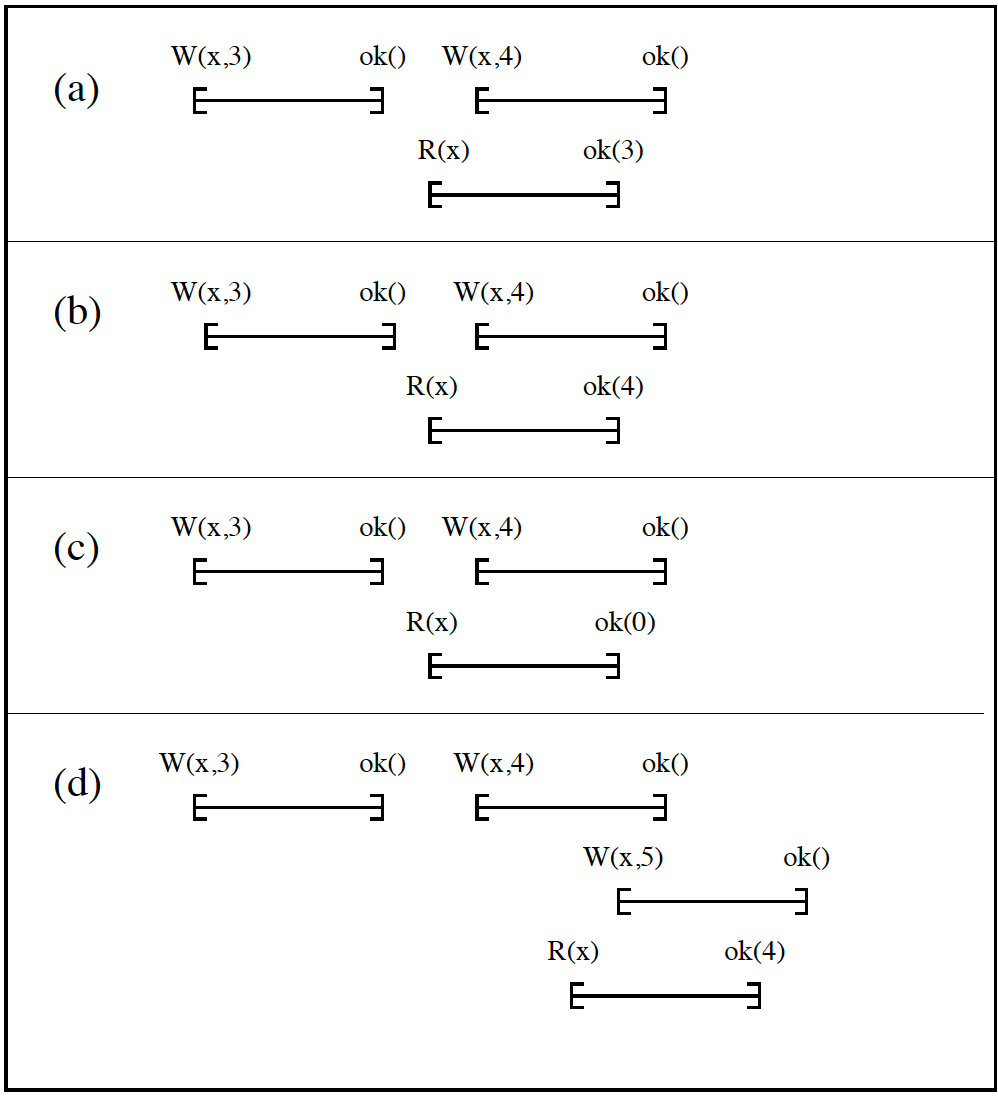
\includegraphics[width=4.5in]{q1.png}
\end{center}
Which register is \emph{safe} in the figure above?
\begin{enumerate}
\item[A.] (a) 
\item[B.] (a) and (b)
\item[C.] (a),  (b) and (d)
\item[D.] All of above
% Answer: D
\end{enumerate}
Answer: D

\section*{Q2}
\begin{center}
	\centering
	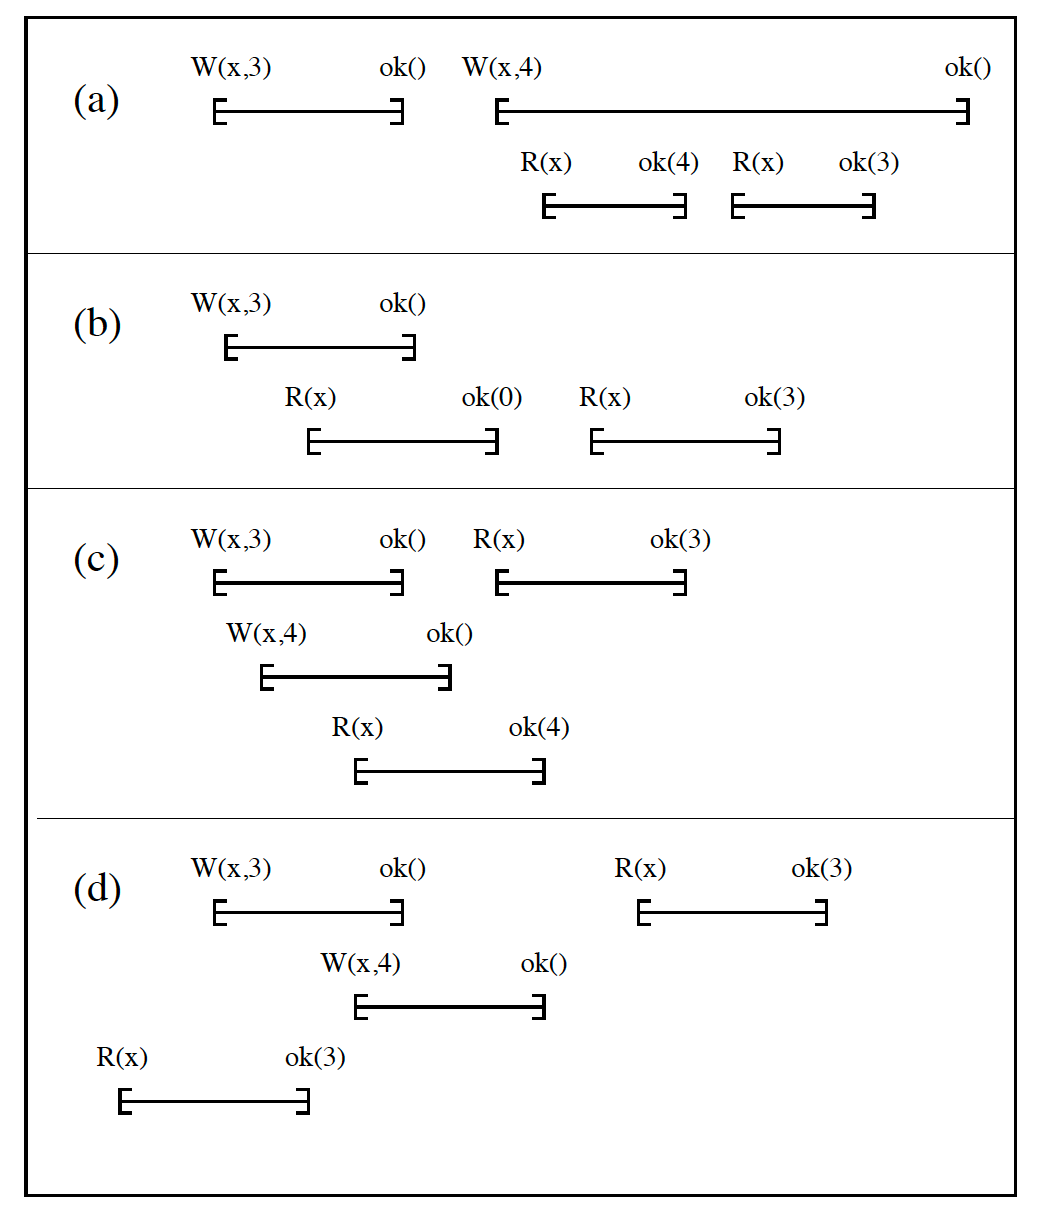
\includegraphics[width=4.5in]{q2.png}
\end{center}
Which register is \emph{regular} in the figure above (The initial value is 0)?
\begin{enumerate}
	\item[A.] (a)
	\item[B.] (a) and (c)
	\item[C.] (a),  (c) and (d)
	\item[D.] All of above
	% 
\end{enumerate}
Answer: D

\section*{Q3}
\begin{center}
	\centering
	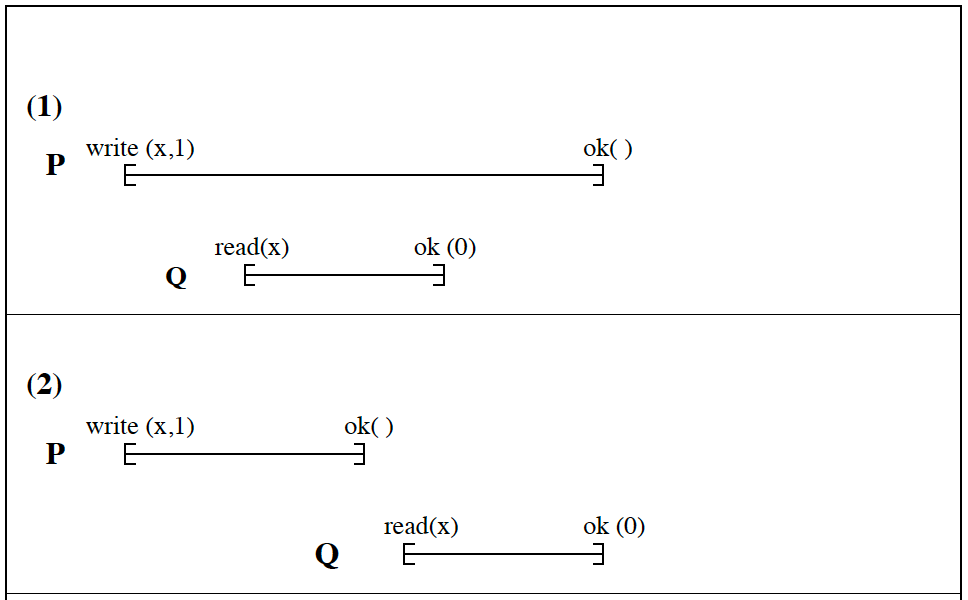
\includegraphics[width=4.5in]{q3.png}
\end{center}
Which register is \emph{atomic} in the figure above (The initial value is 0)?
\begin{enumerate}
	\item[A.] (1)
	\item[B.] (2)
	\item[C.] Both
	\item[D.] Neither
\end{enumerate}
	Answer: A

\section*{Q4}
Consider the following concurrent program:\\
Initially, a = 0, b = 0\\
P1: a = 1; print a; print b;\\
P2: b = 2; print a; print b;\\
Assume the output is P1: 12, P2: 02;
Is it possible for both of the two to be atomic? If possible, please give a history to show that.\\

Answer: it's possible for the following sequence:\\
P2(w b 2) - P2(r a 0) - P2(r b 2) - P1(w a 1) - P1(r a 1) - P2(r b 2),\\
which is linearizable, so both a and b are atomic.

\section*{Q5}
Briefly introduce the key method which is use to construct from \textit{SRSW safe} bit to \textbf{SRSW }regular bit then to \textbf{SRSW} Multivalued Register?\\

Answer: from SRSW safe, we add a \textit{prev} field to help check, and from SRSW regular to SRSW multivalue, we use a array from 0 to maxVal to allow values in the range 0 ... maxVal-1.

\section*{Q6}
Briefly explain to construct the multi-value SRSW register, why we need to double scan when read?\\

Answer: the aim is to guarantee the linearizability. For example, if we set a[1] and then a[4], and then set 1 false, if we have two read occur sequentially, it may read 4 first and then read 1, which is not allow for a linearizable register. 

\section*{Q7}
Why we need communication matrix to implement the MRSW register?\\

Answer: it essentially allows each register to share information. Comm[i][j] is used by the reader i to inform the value it read to the reader j, so that j will not read the value before the reader i read.

\section*{Q8}
Which algorithm we have learned before can help us to help MRMW register to decide on timestamps?

Answer: Lamport's Bakery Algorithm. 
\section*{References}
\beginrefs
\bibentry{1}{\sc V.K. Garg},  Introduction to Multicore Computing
\endrefs


\end{document}





